
\subsection{Positioning algorithms}


\subsubsection{Ecolocation} \label{ecolocation}

Ecolocation\cite{Ecolocation} is a technique which uses RF and distance
to work out the location of a node in a Wireless Sensor Network (WSN).
They use sense and match system, where the unknown node listens for
packets from all the reference nodes. It orders the packets in the
distance it has travelled, and then try and match it to known distance
orders. 

In an ideal scenario the Relative Signal Strength (RSS) reading from
each reference node would be an accurate indication of the distance
between the node and receiver. By ranking the sequence of RSS readings we can
find a constrain on the location of the unknown node. By having multiple
reference nodes we are increasing the constraints to find the unknown
node. By having fixed reference node locations and with the sequence order
of the RSS reading, we can create constraints to help us determine the location of the unknown
node. The unknown node location estimate can be obtained
by comparing the constraints obtained from RSS measurements to the
constraint sets of each location grid-point and picking the location
which satisfies the maximum number of constraints. If there are more
than one such locations then their centroid is the location estimate.

However in a real world presence of multi-path fading and shadowing
in the RF channel impacts the RSS reading greatly. We would assume
that reference nodes that are far from the unknown node should measure
lower RSS values than the nodes that are near to it. However due to
multi-path fading this is not always true. The percentage of error,
depends on the RF channel condition and the topology and the number
of reference nodes. Tests show that Ecolocation is robust to multi-path
effects of RF channel to some degree. The technique can eradicate
the errors due to random variation in RSS measurements up to a tolerance
level of \left|R\textsubscript{i}-R \textsubscript{j}\right| $
due to the way
its constructed.

Experimental results done by Yedavalli, K. and Krishnamachari, B.
et all shows that localization techniques are more accurate for relatively
clutter free RF channel environments i.e outdoors with a clear line
of sight. Their research also concluded that a single localization
methods does not provide sufficient accuracy for all their unknown
nodes, they recommend a hybrid localization techniques using the
RF channel and node deployment parameters would proved a better accuracy.
They have also not taken any complexity into account, using Ecolocation
would require a large amount of ``offline'' work where you would
have to go through different locations in the space to calculate the
RSS readings at that location and save those readings. This would
be a resource intensive and time consuming operation making it not
ideal in a system mainly targeting mobile devices.


\subsubsection{Trilateration} \label{trilateration_section}
Another technique that is widely used for positioning through RF signals is called Trilateration. Trilateration estimates the position of the receiver by using the strength of signals received from multiple non-collocated, non- collinear transmitters\cite{trilat-characteristics}. Generally this technique is called Multilateration. To get the position estimate in \textit{n} dimensions we need \textit{n+1} transmitters, i.e to get a 2D position estimate we need 3 transmitters. Its called Trilateration when we use three transmitters.

Using the relation between signal strength and distance shown in \eqref{distance_formulae} and estimate of the distance between the device and each transmitter can be obtained.
\begin{figure}[h]
\begin{equation} \label{distance_formulae}
\centering
a = b+20\times log(\lambda/4 \pi) + 10\timesn\times log(1/d)
\end{equation}
\begin{tabular}{@{}>{$}l<{$}l@{}}
    a & power at the receiver\\
    b & transmitter power (in dBm)\\
    \lambda &  wavelength\\
    n & path loss exponent (n = 2 in free space)\\
    d & is the distance between the transmitter and receiver
  \end{tabular}
\end{figure}
\begin{figure}
\centering
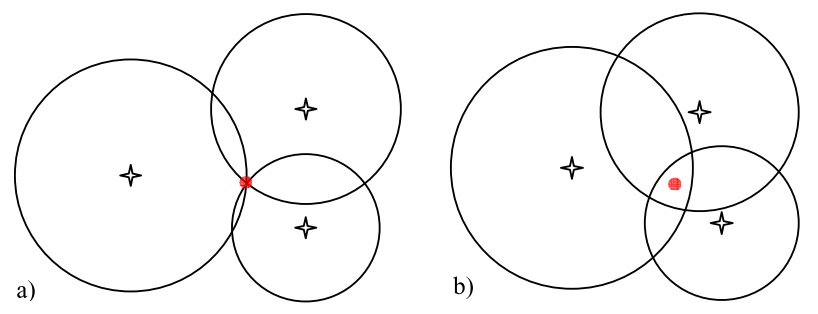
\includegraphics[scale=0.5]{trilat}
\caption{a- shows when there is perfect information, b- shows when there is imperfect information}
\label{trilat_image}
\end{figure}
With perfect information we are able to calculate an exact unique position for the receiver. However we are more likely to get imperfect information which means the circles might not meet at a unique position. In such scenario we use a point that simultaneously minimises the distance to all circles. Figure \ref{trilat_image} shows both scenarios.
\begin{figure}[H]
\begin{lstlisting}[caption = {Algorithm for Trilateration\cite{sig-cart}},frame=single,mathescape, captionpos=b,numbers=left,numbersep=5pt,label={psuedo-code}]
Input: Array of APs: ap_list
Input: Array of Floats: distance_list
Input: Point: min
Input: Point: max
Input: Float: step
Integer: nb_ap  ap_list.size()
Float: d_min <- $\infty$
Float: xm <- x <- minx
Float: ym <- y <- miny
while x <= maxx do
    y <- miny
    while y <= maxy do
        Float: d_max <- 0
        for i <- 0 to nb_ap do
            if distance(x, y, ap_list[i], distance_list[i]) > d_max then
                d_max <- distance(x, y, ap_list[i], distance_list[i])
            end if
        end for
        if d_max <= d_min then
            d_min <- d_max
            xm <- x
            ym <- y
        end if
        y<- y + step
    end while
    x <- x + step
end while
return xm, ym
\end{lstlisting}
\end{figure}

Listing \ref{psuedo-code} shows the psuedo code for trilateration. However Trilateration on its own is not a very good technique to identify the location because imperfect data. \citeauthor{trilat-fusion} recommends we use something else with trilateration for positioning system\cite{trilat-fusion}  such as Ecolocation explained in \ref{ecolocation}.
\subsubsection{Inertial Navigation System (INS)}

INS\cite{innertial_nav_sys} is based on the internal sensors that a devices have
such as Accelerometer, Gyroscope etc. We can use the information from
these sensors to keep track of the position and the orientation of
the mobile device relative to the starting position and orientation
of the device. INS has many uses, including navigation systems for
aircraft and missiles\cite{ins-wiki}.


\paragraph{Accelerometer} \label{accelerometer}

Accelerometer\cite{accl-guide} is a very common sensor that is built into almost
all the mobile devices out there. It measures the proper acceleration
of the device which might not be the same as the coordinate acceleration
(change in velocity over time). Proper acceleration is the weight
experienced by a test mass that which is in the frame of reference
of the accelerometer device. So accelerometer measure how much mass
presses on something when a force acts on it.

Any accelerometer at rest on a surface will show an acceleration of
approximately 1G upwards\cite{accl-wiki}, due to the earths gravitational force. At
any point on earths surface there is an acceleration of 1G upwards
relative to the local frame. This offset has to be subtracted to get
the motion with respect to the Earth. There are many uses for accelerometer such as,
monitoring vibrations and also also used in mobile devices to
keep the images displayed on the screen upright. Highly sensitive
accelerometers are used in drones for flight stabilisation.

Mobile devices are usually equipped with a multi-axis models of accelerometers,
which can detect magnitude and direction of acceleration as
vector quantity. They can then be used to work out the displacement
of a device. However the accelerometers used by the android devices
are not very accurate, therefore there is a lot of noise and calibration
steps required before hand by the user to get a acceptable results.

\begin{figure}[H]
\[
x=\int\int a\mathrm{\text{ }d}t
\]
 

\protect\caption{Acceleration to displacement}


\end{figure}



\paragraph{Gyroscope}

Gyroscope\cite{innertial_nav_sys} is a sensor for measuring and determining the orientation
of a device. This is done be using the principles of conservation
of angular momentum. A gyroscope usually consist of a free rotating
disk called a rotor mounted on a spinning axes, in center of a large
more stable wheel, which lets it rotate in all the axes. As the axis
turns, the rotor remains stationary to indicate the central gravitational
pull, therefore showing us which way is down.

One of the best examples of reading a gyroscope is the altitude indicator
of an aircraft. It is represented by a circular display divided in
half. The top half is blue indicating the sky and the bottom half
is red to show the ground. As the aircraft banks for a turn, the indicator
with shift to account for the actual direction of the ground.

Gyroscopes are also used in INS. Another advantage of them are, that
you can use them where magnetic compasses don't work such as the Huddle
Telescope\cite{gyroscope-wiki}.

\subsubsection{Filter Methods} \label{filter_methods}


\paragraph{Kalman Filter}
\todo[inline]{do this section}
